% --------------------------------------------------------------
%                           Set Up
% --------------------------------------------------------------
 
\documentclass[12pt]{article}
 
\usepackage[margin=1in]{geometry} 
\usepackage{amsmath,amsthm,amssymb}
\usepackage{listings}
\usepackage{xcolor}
\usepackage{graphicx}
\usepackage{subcaption}
\usepackage{listings}
\usepackage{xcolor}
\usepackage{comment}
\usepackage{hepnames}
\usepackage{longtable}
 
\definecolor{codegreen}{rgb}{0,0.6,0}
\definecolor{codegray}{rgb}{0.5,0.5,0.5}
\definecolor{codepurple}{rgb}{0.58,0,0.82}
\definecolor{backcolour}{rgb}{0.95,0.95,0.92}
 
\lstdefinestyle{mystyle}{
    backgroundcolor=\color{backcolour},   
    commentstyle=\color{codegreen},
    keywordstyle=\color{magenta},
    numberstyle=\tiny\color{codegray},
    stringstyle=\color{codepurple},
    basicstyle=\ttfamily\footnotesize,
    breakatwhitespace=false,         
    breaklines=true,                 
    captionpos=b,                    
    keepspaces=true,                 
    numbers=left,                    
    numbersep=5pt,                  
    showspaces=false,                
    showstringspaces=false,
    showtabs=false,                  
    tabsize=2
}
 
\lstset{style=mystyle}
 
\definecolor{codegreen}{rgb}{0,0.6,0}
\definecolor{codegray}{rgb}{0.5,0.5,0.5}
\definecolor{codepurple}{rgb}{0.58,0,0.82}
\definecolor{backcolour}{rgb}{0.95,0.95,0.92}
\definecolor{deepblue}{rgb}{0,0,0.5}
\definecolor{deepred}{rgb}{0.6,0,0}
\definecolor{deepgreen}{rgb}{0,0.5,0}
 
\lstdefinestyle{mystyle}{
    backgroundcolor=\color{backcolour},   
    commentstyle=\color{codegreen},
    keywordstyle=\color{deepred},
    numberstyle=\tiny\color{codegray},
    stringstyle=\color{deepblue},
    basicstyle=\ttfamily\footnotesize,
    breakatwhitespace=false,         
    breaklines=true,                 
    captionpos=b,                    
    keepspaces=true,                 
    numbers=left,                    
    numbersep=5pt,                  
    showspaces=false,                
    showstringspaces=false,
    showtabs=false,                  
    tabsize=2
}
 
\lstset{style=mystyle}
 
\newcommand{\N}{\mathbb{N}}
\newcommand{\Z}{\mathbb{Z}}
 
\newenvironment{theorem}[2][Theorem]{\begin{trivlist}
\item[\hskip \labelsep {\bfseries #1}\hskip \labelsep {\bfseries #2.}]}{\end{trivlist}}
\newenvironment{lemma}[2][Lemma]{\begin{trivlist}
\item[\hskip \labelsep {\bfseries #1}\hskip \labelsep {\bfseries #2.}]}{\end{trivlist}}
\newenvironment{exercise}[2][Exercise]{\begin{trivlist}
\item[\hskip \labelsep {\bfseries #1}\hskip \labelsep {\bfseries #2.}]}{\end{trivlist}}
\newenvironment{problem}[2][Problem]{\begin{trivlist}
\item[\hskip \labelsep {\bfseries #1}\hskip \labelsep {\bfseries #2.}]}{\end{trivlist}}
\newenvironment{question}[2][Question]{\begin{trivlist}
\item[\hskip \labelsep {\bfseries #1}\hskip \labelsep {\bfseries #2.}]}{\end{trivlist}}
\newenvironment{corollary}[2][Corollary]{\begin{trivlist}
\item[\hskip \labelsep {\bfseries #1}\hskip \labelsep {\bfseries #2.}]}{\end{trivlist}}

\newenvironment{solution}{\begin{proof}[Solution]}{\end{proof}}

\setlength\parindent{0pt}
 
\begin{document}
 
% -------------------------------------------------------------- 
%                         Start here
% --------------------------------------------------------------
 
\title{Homework }
\author{Timothy Holmes\\ %replace with your name
PHY 442 Computational Physics}

\maketitle

\section*{Problem 1}

The initial problem, matrix and vector, are given as the following,

\begin{center}
\begin{bmatrix} 
 2 & -1 &  0 &  0 & 0 \\
 -1 & 2 & -1 &  0 & 0 \\
 0 & -1 &  2 & -1 & 0 \\ 
 0 & 0 & -1 &  2 & -1 \\ 
 0 & 0 &  0 & -1 & 2 \\ 
\end{bmatrix}
\begin{bmatrix} 
x_{1} \\ x_{2} \\ x_{3} \\ x_{4} \\ x_{5} \\
\end{bmatrix}
=
\begin{bmatrix} 
0 \\ 1 \\ 2 \\ 3 \\ 4 \\
\end{bmatrix}.
\end{center}

The prior equation is in the form $Ax = b$ where $A$ is the matrix, $b$ is the vector, and the $x's$ are the unknowns. If we forget about the $x$ values and the $b$ vector for now, the matrix $A$ needs to be reduced in a way where it becomes two different matrices. One will become a lower triangular matrix $L$ and the other will be an upper triangular matrix $U$. To do so, the method of row reduction is used. These steps are quite extended and will be left out as an activity for the grader. After the row reduction, the lower triangular matrix becomes 

\begin{center}
L = 
\begin{bmatrix} 
 1 & 0 & 0 & 0 & 0 \\
 -1/2 & 1 & 0 &  0 & 0 \\
 0 & -0.67 &  1 & 0 & 0 \\ 
 0 & 0 & -0.75 &  1 & 0 \\ 
 0 & 0 &  0 & -0.8 & 1 \\ 
\end{bmatrix}
\end{center}

and the upper triangular matrix becomes

\begin{center}
U = 
\begin{bmatrix} 
 2 & -1 &  0 &  0 & 0 \\
 0 & 1.5 & -1 &  0 & 0 \\
 0 & 0 &  1.33 & -1 & 0 \\ 
 0 & 0 & 0 &  1.25 & -1 \\ 
 0 & 0 &  0 & 0 & 1.2 \\ 
\end{bmatrix}.
\end{center}

Now the both $L$ and $U$ are known, the forward substitution and backward substitution methods can be applied. First, the forward substitution can be found by $Ly = b$. In matrix form this is

\begin{center}
\begin{bmatrix} 
 1 & 0 & 0 & 0 & 0 \\
 -1/2 & 1 & 0 &  0 & 0 \\
 0 & -0.67 &  1 & 0 & 0 \\ 
 0 & 0 & -0.75 &  1 & 0 \\ 
 0 & 0 &  0 & -0.8 & 1 \\ 
\end{bmatrix}
\begin{bmatrix} 
y_{1} \\ y_{2} \\ y_{3} \\ y_{4} \\ y_{5} \\
\end{bmatrix}
=
\begin{bmatrix} 
0 \\ 1 \\ 2 \\ 3 \\ 4 \\
\end{bmatrix}.
\end{center}

The results from this substitution are

\begin{align*}
    y_{1} = 0 \\
    -0.5y_{1} + y_{2} = 1 \rightarrow y_{2} = 1 \\
    -0.67y_{2} + y_{3} = 2 \rightarrow y_{3} = 2.667 \\
    -0.75y_{3} + y_{4}  = 3 \rightarrow y_{4} = 5 \\
    -0.8y_{4} + y_{5} = 4 \rightarrow y_{5} = 8. \\
\end{align*}

Knowing the $y$ values the next part of the process can be solved. The next step is backward substitution where $Ux = y$ in matrix form is 

\begin{center}
\begin{bmatrix} 
2 & -1 &  0 &  0 & 0 \\
 0 & 1.5 & -1 &  0 & 0 \\
 0 & 0 &  1.33 & -1 & 0 \\ 
 0 & 0 & 0 &  1.25 & -1 \\ 
 0 & 0 &  0 & 0 & 1.2 \\ 
\end{bmatrix}
\begin{bmatrix} 
x_{1} \\ x_{2} \\ x_{3} \\ x_{4} \\ x_{5} \\
\end{bmatrix}
=
\begin{bmatrix} 
0 \\ 1 \\ 2.667 \\ 5 \\ 8 \\
\end{bmatrix}.
\end{center}

The results from backward substitution are 

\begin{align*}
    2x_{1} - x_{2} = 0 \rightarrow x_{1} = 3.33 \\
    1.5x_{2} - x_{3} = 1 \rightarrow x_{2} = 6.667 \\
    1.33x_{3} - x_{4} = 2.667 \rightarrow x_{3} = 9 \\
    1.25x_{4} - x_{5} = 5 \rightarrow x_{4} = 9.336 \\
    1.2x_{5} = 8 \rightarrow x_{5} = 6.667 \\
\end{align*}

The matlab program, as shown in the appendix, outputs 

\begin{center}
\begin{lstlisting}[language=Matlab, caption=LU Factor Output]
The x values are:
  -------------  
    x1 = 3.33  
    x2 = 6.67  
    x3 = 9.00  
    x4 = 9.33  
    x5 = 6.67  
  ------------- 
\end{lstlisting}
\end{center}

confirming that out answers are correct.

\newpage

\section*{Problem 2}

Following the exact same approach as Problem 1, the first thing that need to be done is row reducing to find $L$ and $U$. Since this matrix has less zeros this makes this step even longer than the last. Once this is found the equations $Ly = b$ and $Ux = y$ are solved. The matlab program outputs the following

\begin{lstlisting}[language=Matlab, caption=LU Factor Output]
The x values are:
  -------------  
    x1 = 125.00  
    x2 = -2880.00  
    x3 = 14490.00  
    x4 = -24640.00  
    x5 = 13230.00  
  -------------  
 \end{lstlisting}
  
\newpage
  
\section*{Problem 3}

I used my own LUFactorization code for all the problems in the homework assignment test against the LUF20soultion code. Rounding may be different but I can assure the values are similar. The following is the output for problem 3.

\begin{lstlisting}[language=Matlab, caption=General Least Squares Output]
Value of a: 0.140281 
Value of b: 0.009487 
f(v) = 0.140281v + 0.009487v^2 
\end{lstlisting}

\begin{figure}[h!]
    \centering
    {{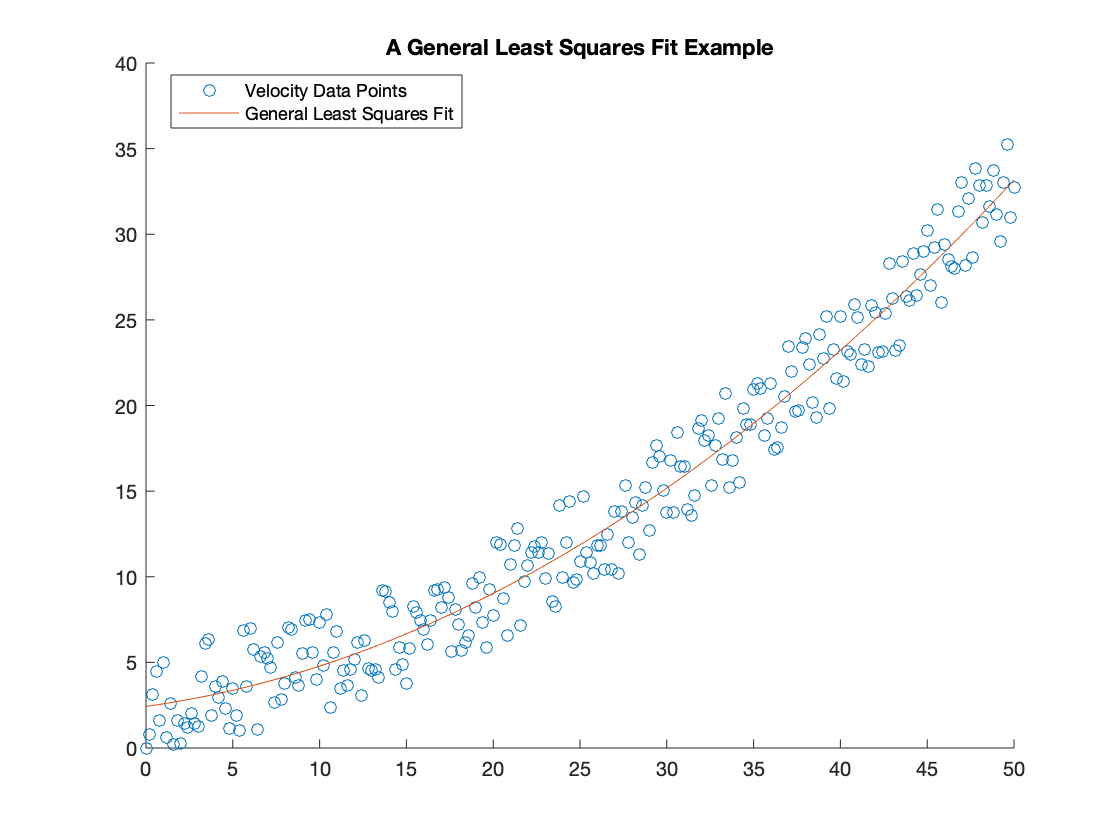
\includegraphics[width=15cm]{figure1.png}}}%
    \qquad
    \caption{ }%
    \label{fig:example}%
\end{figure}

\newpage

\section*{Problem 4}

The following values were used for both methods.


\begin{longtable}{| c | c |}
\hline
a(i) & value \\
A & 7 \\
\mu & 12 \\
\sigma & 1 \\
\hline
\end{longtable}

The code for this problem can be found in the appendix under the name nls\_method\_1. 

\begin{figure}[h!]
    \centering
    {{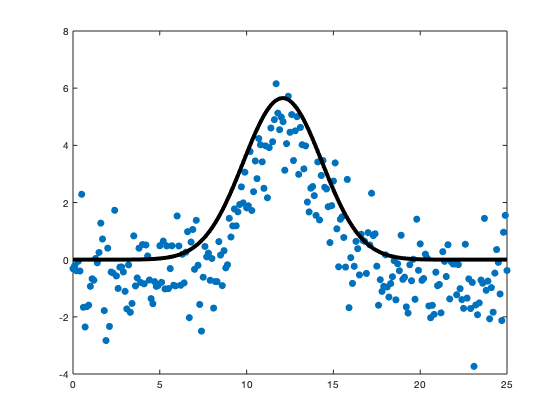
\includegraphics[width=15cm]{nls_method_1.png}}}%
    \qquad
    \caption{Output from the Non-Linear Least Squares Method 1}%
    \label{fig:example}%
\end{figure}

The code for this problem can be found in the appendix under the name nls\_method\_2. 

\begin{figure}[h!]
    \centering
    {{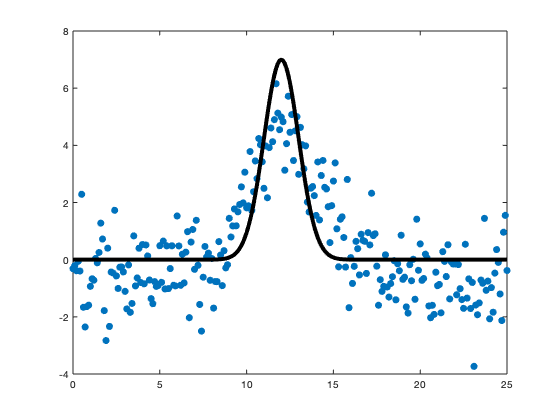
\includegraphics[width=15cm]{nls_method_2.png}}}%
    \qquad
    \caption{Output from the Non-Linear Least Squares Method 2}%
    \label{fig:example}%
\end{figure}

\newpage

\section*{Appendix}

\subsection*{LU Factor Matlab Program}
\begin{lstlisting}[language=Matlab, caption=LU Factor Matlab Program]
function [x] = lu_factorization(A, b)
%% LU Fact
%   - Find unkown x_i values while knowing the
%     matrix and r.h.s array
%   
%   Input Arg
%   ---------
%   A - martix:
%       A general tridiagonal system.
%   r - array:
%       R.H.S values.


if (~exist('A', 'var')) && (~exist('b', 'var'))
    [A, b] = homework_2_values(); 
end

[M, N] = size(A);

if (M ~= N)
    error('Error: Matrix A must be an NxN matrix' );
    return % Kills process
end

%% Prallocate 
L = zeros(N, N); % Lower triangle
U = zeros(N, N); % Upper triangle 

%% LU decomposition
for i=1:N
    %% Fail when any number on the diag = 0 
    if A(i, i) == 0
        warning('LU factorization fails')
        return % Kills process
    else
        %% Find Upper Decomposition
        for k=1:(i - 1)
            L(i, k) = A(i, k);
            for j = 1:(k - 1)
                L(i, k)= L(i, k) - L(i, j) * U(j, k);
            end
            L(i, k) = L(i, k)/U(k, k);
        end
    end

    %% Find Lower Decomposition
    for k = i:N
        U(i, k) = A(i, k);
        for j = 1:(i - 1)
            U(i, k)= U(i, k) - L(i, j) * U(j, k);
        end
    end
    L(i,i)=1;
end

%% Forward Substitution
y = forward_substitution(L, b);  % LY = B

%% Backward Substitution
x = backward_substitution(U, y); % UX = Y

%% Output values
count = 1:length(x);
fprintf("The x values are:\n")
fprintf("  -------------  \n")
fprintf("    x%d = %0.2f  \n", [count(:), x(:)].')
fprintf("  -------------  \n")


end


function [y] = forward_substitution(L, b)

N = size(L, 1);
y(1, :) = b(1, :)/L(1, 1);
for i = 2:N
    y(i, :) = (b(i, :) - L(i, 1:(i - 1)) * y(1:(i - 1), :))/L(i, i);
end

end


function [x] = backward_substitution(U, y)

N = size(U, 2);
U(N,N)
x(N, :) = y(N, :)/U(N, N);
for i = (N - 1):-1:1
    x(i, :) = (y(i, :) - U(i, (i + 1):N) * x((i + 1):N, :))/U(i, i);
end

end


function [A, b] = homework_2_values()
A = [ 2 -1   0   0  0; -1  2  -1   0  0; 0 -1   2  -1  0; 0  0  -1   2 -1; 0  0   0  -1  2;];
b = [0; 1; 2; 3; 4;];

% A = [ 1 1/2 1/3 1/4 1/5; 1/2 1/3 1/4 1/5 1/6; 1/3 1/4 1/5 1/6 1/7; 1/4 1/5 1/6 1/7 1/8; 1/5 1/6 1/7 1/8 1/9;];
% b = [1; 2; 3; 4; 5;];
end
\end{lstlisting}

\subsection*{}
\begin{lstlisting}[language=Matlab, caption=General Least Squares Matlab Program]
function [a, b] = general_least_squares(x_i, y_i, sigma_i)
%% general least squares
%   - Curve fit
%   


if (~exist('x_i', 'var')) && (~exist('y_i', 'var'))
    [x_i, y_i] = homework_2_values(); 
end

N = length(x_i);
M = 3;

if (~exist('sigma', 'var'))
    sigma = 1;
    
elseif (exist('sigma', 'var'))
    sigma = sigma_i;
    
else
    warning('Unexpected Error.')
end


alpha = zeros(M, M);
beta = zeros(M, 1);

for i = 1:M
    beta(i) = sum(y_i .* x_i.^(i - 1))./(sigma.^2);
    for j = 1:M
        
       alpha(i, j) = sum(x_i.^(i + j - 2))./(sigma.^2);
        
    end
end

c = inv(alpha);
sigma_sq = zeros(M, M);
for j = 1:M
    sigma_sq(j, j) = c(j, j);
end

x = lu_factorization(alpha, beta);
f_v = x(1) + (x(2) .* x_i) + (x(3) .* x_i.^2);

hold on
plot(x_i, y_i, 'o')
plot(x_i, f_v)
legend('Velocity Data Points','General Least Squares Fit')
title('A General Least Squares Fit Example')

fprintf('Value of a: %f \n', x(2))
fprintf('Value of b: %f \n', x(3))
fprintf('f(v) = %fv + %fv^2 \n', x(2), x(3))

disp('Done.')
end


function [x_i, y_i, sigma_i] = homework_2_values()

vel_dep_forces = importdata('./vel_dep_forces.dat');

x_i = vel_dep_forces(:, 1);
y_i = vel_dep_forces(:, 2);
sigma_i = 1;

%basis_function = @(x) (a * x) + (b * x^2);

end
\end{lstlisting}

\subsection*{}
\begin{lstlisting}[language=Matlab, caption= ]
function nls_method_1(x, y)
clear;

if (~exist('x', 'var')) && (~exist('y', 'var'))
    [x, y] = homework_2_values(); 
end

a(1) =  7;
a(2) =  12;
a(3) =  1;
h = 0.01;

[a, h, x, y] = crude(a, h, x, y); 

plot(x, y, '.', 'MarkerSize', 18)
hold on

fitf = @(x) a(1) * exp(-((x - a(2)).^2)/(2 * a(3)^2));%function with best fit parameters;
plot(x, fitf(x), '-k', 'LineWidth', 4)

end


function [a,h,x,y] = crude(a, h, x, y) 
%%import the data x, y
for i = 1:length(a) 
    % The SUM will be evaluated with the parameters z
    % A_PLUS, A, and A_MINUS: 
    amax = 100;
    tol = 0.00001;  % used to stop while loop
    ict = 0;
    while amax ~=0
    for k = 1:length(a) 
        if(k == i) 
            a_plus(i)  = a(i) + h; 
            a_minus(i) = a(i) - h;
        else 
            a_plus(k)  = a(k); 
            a_minus(k) = a(k); 
        end 
    end 
    sp = LSE(a_plus, x, y); % Evaluate the sums. 
    s0 = LSE(a, x, y); 
    sm = LSE(a_minus, x, y);
    a1=a(i);
    a(i) = a(i) - 0.5 * h * (sp - sm)/(sp - 2 .* s0 + sm); 
    ict = ict + 1;
    if abs(a(i) - a1) < tol
        amax = 0;
    end
    if ict > 10^4  %taking to long, lets just stop
        amax = 0;
    end
    % As we move towards a minimum, we should decrease 
    % step size used in calculating the derivative. 
    
    h = 0.5 * h; 
    end
end
    
end


function [ss] = LSE(a, x, y) 

% The theoretical curve TC is given as 
%
f_x = @(x) a(1) * exp(-((x - a(2)).^2)/(2*a(3)));

ss = 0.; 
len = length(x);
for i = 1:len 
    % evaluate the theoretical curve: 
    TC = f_x(x(i));
    ss = ss + (y(i) - TC).^2; 
end 

end


function [x, y] = homework_2_values()

gaussian = importdata('./gaussian.dat');
x = gaussian(:, 1);
y = gaussian(:, 2);

end
\end{lstlisting}

\subsection*{}
\begin{lstlisting}[language=Matlab, caption= ]
function nls_method_2(x, y)
clear;

if (~exist('x', 'var')) && (~exist('y', 'var'))
    [x, y] = homework_2_values(); 
end

a(1) =  7;
a(2) =  12;
a(3) =  1;
h = linspace(0.01, 0.05, 3); 

[a, h, x, y] = crude(a, h, x, y); 

plot(x, y, '.', 'MarkerSize', 18)
hold on

fitf = @(x) a(1) * exp(-((x - a(2)).^2)/(2 * a(3)^2));%function with best fit parameters;
plot(x, fitf(x), '-k', 'LineWidth', 4)

end


function [a, h, x, y] = crude(a, h, x, y) 
%%import the data x, y

m = length(a);
hessian = zeros(m, m);

for i = 1:m
    for j = 1:m
        if i==j
            for k = 1:m
                ap(k) = a(k);
                am(k) = a(k);
            end
                ap(i) = a(i) + h(i);
                am(i) = a(i) - h(i);
                hessian(i,i) =(LSE(ap, x, y) -2*LSE(a, x, y)+LSE(am, x, y))/(h(i) *h(i));
        else
            for k = 1:m
                app(k) = a(k);
                apm(k) = a(k);
                amp(k) = a(k);
                amm(k) = a(k);
            end
            app(i) = a(i) + h(i);
            app(j) = a(j) + h(j);
            % amp and amm work similarly
            hessian(i,j) = ((LSE(app, x, y) - LSE(apm, x, y))/(2*h(j))-...
                (LSE(amp, x, y)-LSE(amm, x, y))/(2*h(j)))/(2*h(i));
            hessian(j,i) = hessian(i,j);
        end
    end
end


%x = lu_factorization(hessian, a);
delta = LUF20solve(hessian, a, 3);
fprintf('%f', x)


for i = 1:m
    if delta(i) > 0.001
        a(i) = a(i) + delta(i);
    else
        delta(i) = 0;
    end
end

end


    

function [ss] = LSE(a, x, y)

% The theoretical curve TC is given as 
% a(1) *exp(-(x(i)-a(2)).^2/(2*a(3)))
ss = 0.; 
len = length(x);
for i = 1:len 
   % evaluate the theoretical curve: 
   TC= a(1) *exp(-(x(i)-a(2)).^2/(2*a(3)));   %??
   ss=ss+(y(i)-TC).^2; 
end 
end


function [x, y] = homework_2_values()

gaussian = importdata('./gaussian.dat');
x = gaussian(:, 1);
y = gaussian(:, 2);

end
\end{lstlisting}


% --------------------------------------------------------------
%                           End Document.
% --------------------------------------------------------------
 
\end{document}

